\documentclass[WHATMANUAL.tex]{subfiles}

\begin{document}

\chapter{Projects Management in WHAT}\label{WHAT_projects}

\section{Introduction}

Data is managed in WHAT by project. That is all input and output files relative to a given project are saved within a common folder called the ``project folder''. This file management system allows you to easily backup and move your projects from one location to the other since all the files relating to a given project are saved at the same place. 

On first launch, WHAT will automatically open an example that is distributed with the software with all the necessary files to easily and quickly test the functionality of the program. The title of the currently opened project is shown in the menu bar at the top of the interface. Additional information about the project can be displayed by clicking on the small ``i'' icon located next to the project name. There can be only one opened project at a time per instance of WHAT. 

\section{Create a New Project}

To start a new project, click on the button \textsl{New Project\dots} with the small folder icon located at the right end of the WHAT menu bar (see Figure~\ref{fig:WHAT_GUI}). This will open a new dialog window (see Figure~\ref{fig:new_proj_win}) where you can enter various information about your project such as its title, author and location coordinates. 

Clicking on the button \textsl{Save} creates a new project folder named after your project title in which your project information are saved in a file with a ``.what'' extension. The new folder is created in the location defined by the \textsl{Save in Folder} directory path. For example, saving the \textsl{My New Project} of Figure~\ref{fig:new_proj_win} would create a folder named ``My New Project'' in the directory ``\textsl{C:\textbackslash{}Users\textbackslash{}johndoe\textbackslash{}WHAT\_4.0.5-beta\textbackslash{}Projects}'' and would saved the project information in the file named ``my\_new\_project.what''. It is possible to change the directory where the project folder is created by clicking the small folder icon located next to the \textsl{Save in Folder} directory path.

\begin{figure}[!ht]
\centering
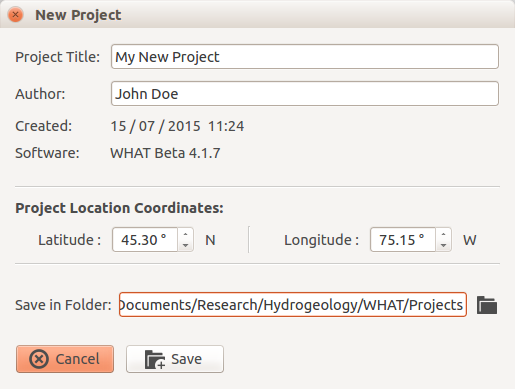
\includegraphics[width=0.5\textwidth]{img/WHAT_Screenshot_newproject}
\caption[New Project dialog window.]{New Project dialog window.}
\label{fig:new_proj_win}
\end{figure}

\FloatBarrier

\section{Open a Project}

To open a new project, click on the name of the currently opened project in the menu bar at the top of WHAT window. This will open a new dialog window where you can browse your folders to select an already existing project file (*.what), and then click Open. WHAT will then open the project and the currently opened project displayed in the menu bar should change to the name of the project you just selected.

The path to your project folder is stored in WHAT in a relative format. This means that if you change the location of your project folder relative the ``WHAT.exe'', your will have to redirect WHAT to the new location of your project by repeating the procedure described in the paragraph above.

\section{Project Folder Structure Overview}\label{subsec:folder_structure}

In addition to the project file (.what file extension) that is created when saving a new project, WHAT automatically generates various files and sub-folders that are required for it to run. This file organization is briefly described here and an example is presented in Figure~\ref{fig:proFolder_organization}. The project folder contains two sub-folders named ``Meteo'' and ``Waterlvl'' in addition to a few other files.

\paragraph{Meteo} The folder \emph{Meteo} contains three sub-folders named respectively Raw, Input and Output. The folder \textbf{Raw} is where are saved the weather data files downloaded from the CDCD. These are coma-separated values (CSV) files that contain weather data on a yearly basis. All the data files for a given weather station are saved within a common folder named after the station name and its unique identification number (IDN). For example, in Figure~\ref{fig:proFolder_organization}, the raw data file ``eng-daily-01011980-12311980.csv'' that contains weather data of the station ``Marieville'' for the year 1980 is saved within a folder named ``MARIEVILLE (7024627)'' where the number in parentheses is the unique IDN of the station.

The folder \textbf{Input} contains the formatted weather data files produced from the raw data files. These are tab-separated values (TSV) files that are named after the station's name and IDN.

The folder \textbf{Output} is where are saved the gapless weather time-series produced from the content of the Input folder. These are saved in TSV text files with the extension ``.out''. The files with the extension ``.log'' are TSV text files that contain detailed information about every missing daily weather value that were estimated by the program to produce the gapless time-series (.out files).

\paragraph{Waterlvl} The folder ``Waterlvl'' is the preferred location were your water level time-series should be stored. These files can be  either in a Microsoft Excel spreadsheet file format (xls) or in a tab-separated values text format (TSV).

\paragraph{Other Files} The file ``weather stations.lst'' is a resource file that is used to store the results of a weather station search in the Canadian Daily Climate Database (CDCD). The file ``graph layout.lst'' is also a resource file in which are stored the layout parameters of the well hydrographs that are produced in the hyhdrograph tab of WHAT. The file ``STATION SUMMARY.log'' is an tab-separated values (TSV) file that contains a summary of all the weather data files contained in the ``Input'' folder. The file ``waterlvl manual measurements.xls'' is used to input manual water level measurements associated with the water level time-series files stored in the ``Waterlvl'' folder. These measurements are plotted on the hydrograph and can also be used to adjust the position of the water-level time-series in the vertical axis when the installation depth of the pressure probe is unknown.\vspace{1cm}

\begin{figure}[!ht]
\centering
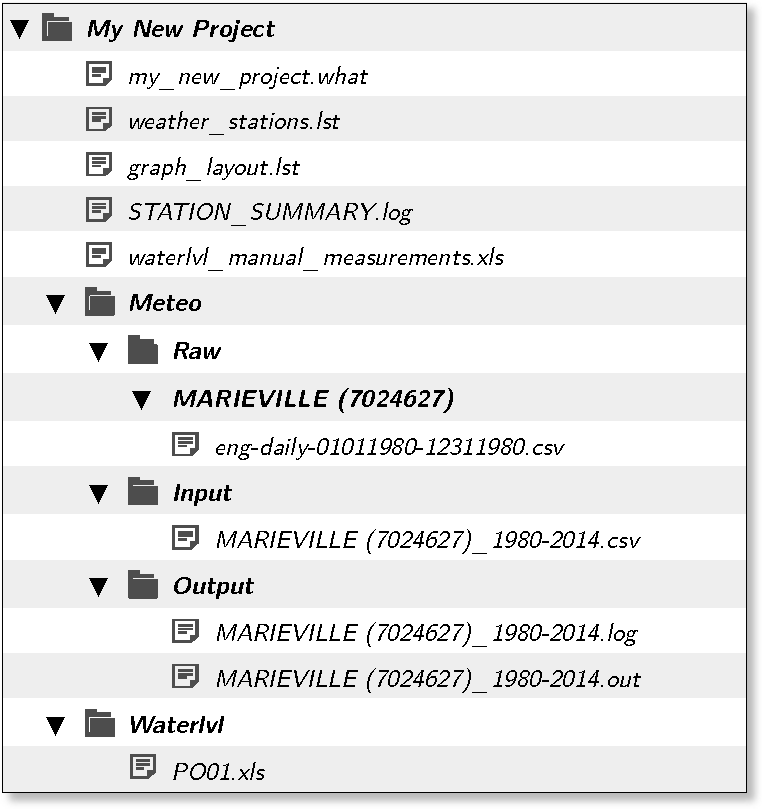
\includegraphics[width=0.5\textwidth]{img/file_and_folder_architecture}
\caption[Project folder file organization.]{Project folder file organization.}
\label{fig:proFolder_organization}
\end{figure}

\FloatBarrier

\end{document}